\section[PKI and blockchains]{Background on public key infrastructure (PKI) and blockchains}

\begin{frame}{Public key infrastructure}
A \mg{public key infrastructure (PKI)} is a set of roles, policies, and procedures needed to create, manage, distribute, use, store, and revoke digital certificates and manage public-key encryption.

\vspace{2mm}

PKI involves
\begin{itemize}
\item public key cryptography,
\item digital certificates,
\item digital identity management.
\end{itemize}

\end{frame}


\begin{frame}{Public key infrastructure}
\begin{figure}[t]
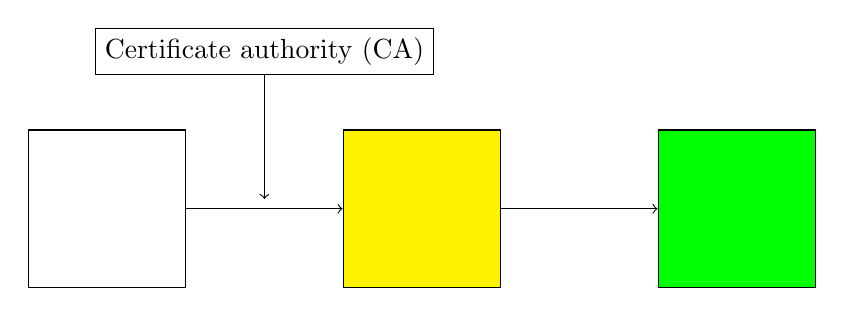
\begin{tikzpicture}
\node[draw,rectangle,
inner xsep=1cm,inner ysep=1cm,
fill=white](user) at (-30,0){};

\node[] (fake) at (-28,0){};

\node[draw,rectangle,
fill=white](ca) at (-28,2){Certificate authority (CA)};

\node[draw,rectangle,
inner xsep=1cm,inner ysep=1cm,
fill=yellow](cert) at (-26,0){};

\node[draw,rectangle,
inner xsep=1cm,inner ysep=1cm,
fill=green](repo) at (-22,0){};


\draw [->] (user) to (cert);
\draw [->] (cert) to (repo);
\draw [->] (ca) to (fake);
\end{tikzpicture}
\end{figure}

a figure to be placed here, based on IDNOMIC's page 6
\end{frame}


\begin{frame}{Public key infrastructure}

certificates, chain of trust

\end{frame}

\begin{frame}{Blockchain definition}

\begin{itemize}
\item A \mg{blockchain} is a public, transparent,
append-only ledger
%\pause
\item Records stored in the ledger are immutable
and unforgeable
\item Created by members of a peer-to-peer
network
\item FunFact
\end{itemize}

\end{frame}



\begin{frame}{Blockchain structure}

\begin{itemize}
\item ssss
\item transactions are validated and broadcast
\item multiple validated transactions
constitute a block, blocks are linked together,
forming a chain
\item the choice of the next blocks to be
added to the chain is a result of a consensus
process
\end{itemize}

\end{frame}
